%%
%
% ARQUIVO: main.tex
%
% VERSÃO: 0.1
% DATA: Novembro de 2016
% AUTOR: Coordenação PPgSC
% 
%  Arquivo tex principal do documento de Dissertação.
%  Este arquivo SÓ PRECISA SER MODIFICADO NA PARTE DE CONTEÚDO:
%
%    a. colocar um \include{•} para cada capítulo da Dissertação.
%
%%

% -----
% CLASSE DO DOCUMENTO DA PROPOSTA DE DISSERTAÇÃO
% -----
\documentclass{proposta}

% -----
% PACOTES LATEX USADOS NO DOCUMENTO DA PROPOSTA DE DISSERTAÇÃO
% -----
\usepackage[brazilian]{babel}
\usepackage[utf8]{inputenc}
\usepackage[T1]{fontenc}

\usepackage{amsmath}
\usepackage{graphicx}
\usepackage{tabularx}
\usepackage{float}
\usepackage{color}
\usepackage{amsfonts,amssymb}
\usepackage[authoryear]{natbib}

\usepackage{enumitem}
\usepackage{rotating}
\usepackage{lipsum}
\usepackage{lastpage}
\usepackage{stringstrings}
\usepackage{pgffor}

% -----
% MARGENS DO DOCUMENTO DA PROPOSTA DE DISSERTAÇÃO
% -----
\usepackage{geometry}
\geometry{
	a4paper,
	total={210mm,297mm},
	left=25mm,
	right=25mm,
	top=25mm,
	bottom=30mm,
	textwidth=160mm,
	textheight=242mm,
	headheight=0mm,
	headsep=0mm,
}

% -----
% DECLARAÇÕES AUXILIARES PARA REFERÊNCIAS
%
%  Diferencia \citet e \citep de acordo com a NBR 10520:2002
% -----
\DeclareRobustCommand{\NATand}{;}
\DeclareRobustCommand{\NATetal}{et~al.}
\makeatletter
\renewcommand{\NAT@nmfmt}[1]{%
  \ifNAT@swa\expandafter\MakeUppercase
  \else\DeclareRobustCommand{\NATand}{ e}\expandafter\@firstofone\fi{{\NAT@up #1}}%
}
\makeatother

% -----
% AMBIENTE DE FIGURAS DA PROPOSTA DE DISSERTAÇÃO
%
%  A classe do documento está configurada SOMENTE para figuras no formato EPS.
%  Logo, use PREFERENCIALMENTE este tipo de arquivo.
%
%    a. os arquivos das figuras devem estar no diretório 'img'
% -----
\graphicspath{{./img/}}

% -----
% INÍCIO DO DOCUMENTO DA PROPOSTA DE DISSERTAÇÃO
% -----
\begin{document}

% -----
% DADOS DA PROPOSTA DE DISSERTAÇÃO
%  ALTERAR o arquivo dados-proposta.tex
% -----
%%
%
% ARQUIVO: dados-proposta.tex
%
% VERSÃO: 1.1
% DATA: Janeiro de 2016
% AUTOR: Coordenação PPgSC
% 
%  Arquivo tex com os dados acerca da Proposta de Dissertação.
%
%
%%

%%% AUTOR DA PROPOSTA DE DISSERTAÇÃO (Nome completo)
\autor{Ricardo de Azevedo Brandão}

%%% CÓDIGO DO AUTOR DA PROPOSTA DE DISSERTAÇÃO
\codigoautor{SC 16113}

%%% POSTO DO AUTOR DA PROPOSTA DE DISSERTAÇÃO
% ---
%  se o autor é CIVIL, REMOVA ESTA LINHA
%  se o autor é MILITAR, coloque CORRETAMENTE o POSTO aqui
% ---
%\postoautor{1 Ten}

%%% TITULO DA PROPOSTA DISSERTAÇÃO
\titulo{Mineração de Dados Distribuída Aplicada à Detecção de Desvios Comportamentais no Contexto da Internet das Coisas}

%%% DATA DA APRESENTAÇÃO (formato {dd}{Mmmmm}{aaaa})
\dataapresentacao{13}{dezembro}{2016}

%%% ÁREA DE CONCENTRAÇÃO DA PROPOSTA DISSERTAÇÃO
% ---
%  VER SITE do PPGSC para ver as Áreas de Concentração do Programa.
%  Em 2016 só existe uma Área de Concentração:
%     Ciência da Computação
% ---
\area{Sistemas e Computação}

%%% LINHA DE PESQUISA DA PROPOSTA DISSERTAÇÃO
% ---
%  VER SITE do PPGSC para ver as Linhas de Pesquisa do Programa.
%  Em 2016 só existem três Linhas de Pesquisa:
%     Metodologia da Computação
%     Sistemas de Computação
%     Engenharia de Sistemas e Informação
% ---
\linha{Engenharia de Sistemas e Informação}

%%% ORIENTADOR DA PROPOSTA DE DISSERTAÇÃO
% ---
%  CAMPO 1: Nome completo
%  CAMPO 2: D (para D.Sc.); P (para Ph.D.); ou qualquer coisa (inclusive VAZIO) - o que for escrito aparecerá no documento
% ---
\orientador{Ronaldo Ribeiro Goldschmidt}{D}

%%% POSTO DO ORIENTADOR DA PROPOSTA DE DISSERTAÇÃO
% ---
%  se o orientador é CIVIL, REMOVA ESTA LINHA
%  se o orientador é MILITAR, coloque CORRETAMENTE o POSTO aqui:
%     pode ser: 1 Ten; Cap; Maj; Ten Cel; Cel
% ---
%\postoorientador{Ten Cel}

%%% CO-ORIENTADOR DA PROPOSTA DE DISSERTAÇÃO
% ---
%  se NÃO HOUVER co-orientador, REMOVA ESTA LINHA
%  preenchimento idêntico a \orientador{}{}
% ---
%\coorientador{Nome Completo do Co-orientador}{P}

%%% POSTO DO CO-ORIENTADOR DA PROPOSTA DE DISSERTAÇÃO
% ---
%  se NÃO HOUVER co-orientador, REMOVA ESTA LINHA
%  caso contrário
%    se o co-orientador é CIVIL, REMOVA ESTA LINHA
%    se o co-orientador é MILITAR, coloque CORRETAMENTE o POSTO aqui:
%       pode ser: 1 Ten; Cap; Maj; Ten Cel; Cel
% ---
%\postocoorientador{Cap}

%%% COORDENADOR DE PÓS-GRADUAÇÃO
% ---
%  CAMPO 1: Nome completo
%  CAMPO 2: D (para D.Sc.); P (para Ph.D.); ou qualquer coisa (inclusive VAZIO) - o que for escrito aparecerá no documento
% ---
\coord{Ronaldo Moreira Salles}{P}

%%% POSTO DO COORDENADOR DE PÓS-GRADUAÇÃO
% ---
%  se o Coordenador de PG é CIVIL, REMOVA ESTA LINHA
%  se o Coordenador de PG é MILITAR, coloque CORRETAMENTE o POSTO aqui:
%     pode ser: 1 Ten; Cap; Maj; Ten Cel; Cel
% ---
\postocoord{Cel}

%%% CHEFE DA SEÇÃO (SE/8)
\chefe{Luiz Henrique da Costa Araújo}

%%% POSTO DO CHEFE DA SEÇÃO (SE/8)
% ---
%  se o Chefe é CIVIL, REMOVA ESTA LINHA
%  se o Chefe é MILITAR, coloque CORRETAMENTE o POSTO aqui:
%     pode ser: 1 Ten; Cap; Maj; Ten Cel; Cel
% ---
\postochefe{Cel}



% -----
% PARTE PRÉ-TEXTUAL DA PROPOSTA DE DISSERTAÇÃO
% -----
\makecapa
\maketitle

\parindent 0.75cm


% -----
% PARTE DE CONTEÚDO DE SUA PROPOSTA DE DISSERTAÇÃO
%
% Alterar o conteúdo dos arquivos capitulo-02.tex / capitulo-03.tex / capitulo-04.tex
% -----
% -----
% ARQUIVO: capitulo-02.tex
% VERSÃO: 1.1
% DATA: Janeiro de 2016
%
% CAPÍTULO DE INTRODUÇÃO DA PROPOSTA
%
% NÃO MEXA NAS SEÇÕES, SOMENTE EDITE O CONTEÚDO.
% -----

\chapter{Introdu\c{c}\~{a}o}
% #TXT_INTRODUCAO
Lorem ipsum dolor sit amet, consectetuer adipiscing elit. Ut purus elit, vestibulum ut, \citep{Ashton2009} placerat ac, adipiscing vitae, felis \citep{Salles2014}. Curabitur dictum gravida mauris. Nam arcu libero, nonummy eget, consectetuer id, vulputate a, magna. Donec vehicula augue \citep{Mashayekhi2015} eu neque. Pellentesque habitant morbi tristique senectus et netus et malesuada fames ac turpis egestas. Mauris ut leo. Cras viverra metus rhoncus sem. Nulla et lectus vestibulum urna fringilla ultrices. Phasellus eu tellus sit amet tortor gravida placerat. Integer sapien est, iaculis in, pretium quis, viverra ac, nunc.

Praesent eget sem vel leo ultrices bibendum. Aenean faucibus. Morbi dolor nulla, malesuada eu, pulvinar at, mollis ac, nulla. Curabitur auctor semper nulla. Donec varius orci eget risus. Duis nibh mi, congue eu, accumsan eleifend, sagittis quis, diam \citep{Justel2014}. Duis eget orci sit amet orci dignissim rutrum. Nam dui ligula, fringilla a, euismod sodales, sollicitudin vel, wisi. Morbi auctor lorem non justo. Nam lacus libero, pretium at, lobortis vitae, ultricies et, tellus. Donec aliquet, tortor sed accumsan bibendum, erat ligula aliquet magna, vitae ornare odio metus a mi. Morbi ac orci et nisl hendrerit mollis. Suspendisse ut massa.

\section{Motiva\c{c}\~{a}o}
% #TXT_MOTIVACAO
Segundo \citet{Goldschmidt2005}, cras nec ante. Pellentesque a nulla. Cum sociis natoque penatibus et magnis dis parturient montes, nascetur ridiculus mus. Aliquam tincidunt urna \citep{Rakocevic2014}. Nulla ullamcorper vestibulum turpis. Pellentesque cursus luctus mauris. Nulla malesuada porttitor diam. Donec felis erat, congue non, volutpat at, tincidunt tristique, libero. Vivamus viverra fermentum felis. Donec nonummy pellentesque ante. Phasellus adipiscing semper elit. Proin fermentum massa ac quam \citep{Lara2014}. Sed diam turpis, molestie vitae, placerat a, molestie nec, leo. Maecenas lacinia. Nam ipsum ligula, eleifend at, accumsan nec, suscipit a, ipsum.

Morbi blandit ligula feugiat magna. De acordo com  \citet{Soares2013} nunc eleifend consequat lorem. Sed lacinia nulla vitae enim. Pellentesque tincidunt purus vel magna. Integer non enim. Praesent euismod nunc eu purus. Donec bibendum quam in tellus \citep{Yoko2003}. Nullam cursus pulvinar lectus. Donec et mi. Nam vulputate metus eu enim. Vestibulum pellentesque felis eu massa. Quisque ullamcorper placerat ipsum. Cras nibh. Morbi vel justo vitae lacus tincidunt ultrices. Lorem ipsum dolor sit amet, consectetuer adipiscing elit. In hac habitasse platea dictumst. Em \citet{Dias2013} integer tempus convallis augue. Etiam facilisis. Nunc elementum fermentum wisi. Aenean placerat.

\subsection{Caracteriza\c{c}\~{a}o do Problema}
% #TXT_PROBLEMA
Ut imperdiet, enim sed gravida sollicitudin, felis odio placerat quam, ac pulvinar elit purus eget enim \citep{Gubitoso1992}. Nunc vitae tortor. Proin tempus nibh sit amet nisl. Vivamus quis tortor vitae risus porta vehicula. Fusce mauris. Vestibulum luctus nibh at lectus. Sed bibendum, nulla a faucibus semper, leo velit ultricies tellus, ac venenatis arcu wisi vel nisl \citep{icse2015}. Aliquam pellentesque, augue quis sagittis posuere, turpis lacus congue quam, in hendrerit risus eros eget felis. Maecenas eget erat in sapien mattis porttitor. Vestibulum porttitor. Nulla facilisi. Sed a turpis eu lacus commodo facilisis. Morbi fringilla, wisi in dignissim interdum, justo lectus sagittis dui, et vehicula libero dui cursus dui.


% -----
% ARQUIVO: capitulo-03.tex
% VERSÃO: 1.1
% DATA: Janeiro de 2016
%
% CAPÍTULO DE CONCEITOS BÁSICOS DA PROPOSTA
%
% NÃO MEXA NAS SEÇÕES, SOMENTE EDITE O CONTEÚDO.
% -----

\chapter{Conceitos B\'{a}sicos}
% #TXT_CONCEITOS
Mauris tempor ligula sed lacus. Duis cursus enim ut augue. Cras ac magna. Cras nulla. Nulla egestas. Curabitur a leo. Quisque egestas wisi eget nunc. Nam feugiat lacus vel est. Curabitur consectetuer. Gini eect on Secondary school enrollment Lorem ipsum dolor sit amet, consectetuer adipiscing elit. Ut purus elit, vestibulum ut, placerat ac, adipiscing vitae, felis. Curabitur dictum gravida mauris. Nam arcu libero, nonummy eget, consectetuer id, vulputate a, magna . Donec vehicula augue eu neque.


% Para usar figuras, use sempre o mesmo template abaixo. altere somente:
% 1. os parâmetros do comando \includegraphics[width=•]{•} / tamanho e arquivo
% 2. \caption{*} / para colocar o rótulo da figura em *
% 3. \label{*} / para colocar a chamada para a figura no texto em *
%    TODA figura deve ter uma chamada no texto e esta deve ser feita sempre no formato:
%    Figura \ref{•} (p. ex. "Figura \ref{fig:artigo1}")

\begin{figure}[!h]
	\centering
	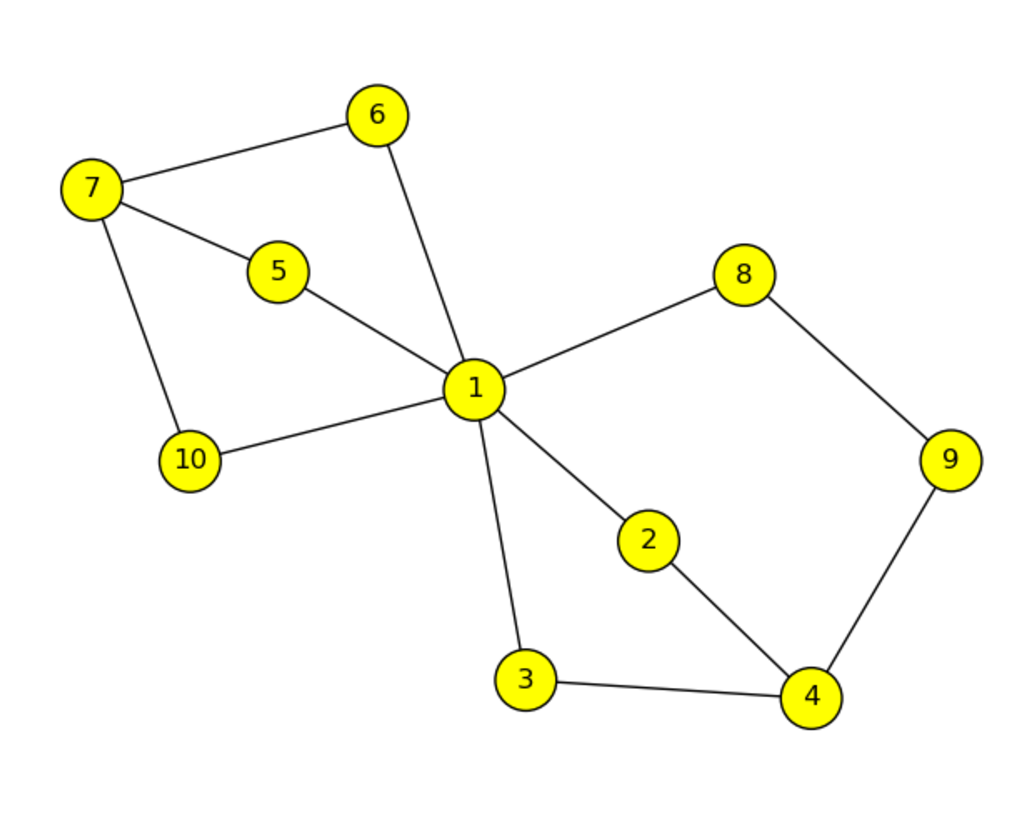
\includegraphics[width=0.4\textwidth]{artigo1.eps}
	\caption{R\'{o}tulo da Figura 1, descrevendo a figura.}
	\label{fig:artigo1}
\end{figure}

Pellentesque habitant morbi tristique senectus et netus et malesuada fames ac turpis egestas, como se pode ver na Figura \ref{fig:artigo1}. Mauris ut leo. Integer sapien est, iaculis in, pretium quis, viverra ac, nunc. Praesent eget sem vel leo ultrices bibendum. Aenean faucibus. Morbi dolor nulla, malesuada eu, pulvinar at, mollis ac, nulla. Sed ut perspiciatis unde omnis iste natus error sit voluptatem accusantium doloremque laudantium, totam rem aperiam, eaque ipsa quae ab illo inventore veritatis et quasi architecto beatae vitae dicta sunt explicabo.

\section{Internet das Coisas}
% #TXT_TRABREL
Cras viverra metus rhoncus sem. Nulla et lectus vestibulum urna fringilla ultrices. Phasellus eu tellus sit amet tortor gravida placerat. Curabitur auctor semper nulla. Donec varius orci eget risus. Duis nibh mi, congue eu, accumsan eleifend, sagittis quis, diam. Duis eget orci sit amet orci dignissim rutrum. Nam dui ligula, fringilla a, euismod sodales, sollicitudin vel, wisi. Morbi auctor lorem non justo. Nam lacus libero, pretium at, lobortis vitae, ultricies et, tellus. Donec aliquet, tortor sed accumsan bibendum, erat ligula aliquet magna, vitae ornare odio metus a mi.

%
% Ambiente de teoremas: \begin{*}
% * pode assumir os seguinte valores:
%	1. thm  - Teorema (na sequência, o texto aparece em itálico)
%	2. prop - Proposição
%	3. defn - Definição (na sequência, o texto aparece em itálico)
%	4. exmp - Exemplo
%	5. nota - Nota
%
\begin{thm}
Um Teorema simples:
\begin{equation}
X^2 := x^2 - 123
\label{thm1}
\end{equation}
\end{thm}

\lipsum[13] 

%
% Referência para um teorema (é igual para todas as opções do ambiente de teoremas)
Conforme o Teorema \ref{thm1}, nemo enim ipsam voluptatem quia voluptas sit aspernatur aut odit aut fugit, sed quia consequuntur magni dolores eos qui ratione voluptatem sequi nesciunt. Neque porro quisquam est, qui dolorem ipsum quia dolor sit amet, consectetur, adipisci velit, sed quia non numquam eius modi tempora incidunt ut labore et dolore magnam aliquam quaerat voluptatem. Ut enim ad minima veniam, quis nostrum exercitationem ullam corporis suscipit laboriosam, nisi ut aliquid ex ea commodi consequatur? Quis autem vel eum iure reprehenderit qui in ea voluptate velit esse quam nihil molestiae consequatur, vel illum qui dolorem eum fugiat quo voluptas nulla pariatur?



% -----
% ARQUIVO: capitulo-04.tex
% VERSÃO: 1.1
% DATA: Janeiro de 2016
%
% CAPÍTULO DE METODOLOGIA DA PROPOSTA
%
% NÃO MEXA NAS SEÇÕES, SOMENTE EDITE O CONTEÚDO.
% -----

\chapter{Abordagem Proposta}
% #TXT_INTROPROPOSTA
\lipsum[1]

\section{Vis\~{a}o Geral}
% #TXT_VISAO_GERAL
\lipsum[1-2]

% PARTE DE QUESTÕES DE PESQUSA - TANTAS QUANTO NECESSÁRIO
\begin{qpesq}
Lorem ipsum dolor sit amet, consectetur adipiscing elit, sed do eiusmod tempor incididunt ut labore et dolore magna aliqua?
\end{qpesq}

\section{Viabilidade}
% #TXT_VIABILIDADE
Quem num gosti di mum que vai caçá sua turmis! Per aumento de cachacis, eu reclamis. Ta deprimidis, eu conheço uma cachacis que pode alegrar sua vidis.” Admodum accumsan disputationi eu sit. Vide electram sadipscing et per.

Nec orci ornare consequat. Praesent lacinia ultrices consectetur. Sed non ipsum felis. Delegadis gente finis, bibendum egestas augue arcu ut est. Posuere libero varius. Nullam a nisl ut ante blandit hendrerit. Aenean sit amet nisi. Suco de cevadiss deixa as pessoas mais interessantiss. 

% -----
% ARQUIVO: capitulo-05.tex
% VERSÃO: 1.0
% DATA: Agosto de 2015
%
% CAPÍTULO DE PLANO DE AÇÃO DA PROPOSTA
%
% NÃO MEXA NAS SEÇÕES, SOMENTE EDITE O CONTEÚDO.
% -----

\chapter{Plano de A\c{c}\~{a}o}
% #TXT_PLANO
\lipsum[1]

\section{Metodologia}
% #TXT_METODOLOGIA
\lipsum[11]

% Para usar tabelas, use sempre o mesmo template abaixo. Altere somente:
% 1. \caption{*} / para colocar o rótulo da tabela em *
% 2. \begin{tabular}{*} / para colocar a formatação da tabela em *
% 3. o conteúdo da tabela (tudo até \end{tabular})

\begin{table}[h]
\centering
\caption{Um nome qualquer}
\vspace{0.5cm}
\begin{tabular}{r|lr}
 
Posi\c{c}\~ao & Pa\'is & IDH \\ % Note a separação de col. e a quebra de linhas
\hline                               % para uma linha horizontal
1 & Noruega        & .955 \\
2 & Austr{\'a}lia  & .938 \\
3 & EUA            & .937 \\
4 & Holanda        & .921 \\
5 & Alemanha       & .920            % não é preciso quebrar a última linha
 
\label{tab:tabela1}
\end{tabular}
\end{table}

At vero eos et accusamus et iusto odio dignissimos ducimus qui blanditiis praesentium voluptatum deleniti atque corrupti quos dolores et quas molestias excepturi sint occaecati cupiditate non provident, similique sunt in culpa qui officia deserunt mollitia animi, id est laborum et dolorum fuga (como mostrado na Tabela \ref{tab:tabela1}). Et harum quidem rerum facilis est et expedita distinctio. Nam libero tempore, cum soluta nobis est eligendi optio cumque nihil impedit quo minus id quod maxime placeat facere possimus, omnis voluptas assumenda est, omnis dolor repellendus. Temporibus autem quibusdam et aut officiis debitis aut rerum necessitatibus saepe eveniet ut et voluptates repudiandae sint et molestiae non recusandae.

\section{Cronograma}
\lipsum[11]

O cronograma para o desenvolvimento das atividades relacionadas a esta proposta pode ser visto na Figura \ref{fig:cronograma}.

% Para usar figuras, use sempre o mesmo template abaixo. altere somente:
% 1. os parâmetros do comando \includegraphics[width=•]{•} / tamanho e arquivo
% 2. \caption{*} / para colocar o rótulo da figura em *
% 3. \label{*} / para colocar a chamada para a figura no texto em *
%    TODA figura deve ter uma chamada no texto e esta deve ser feita sempre no formato:
%    Figura \ref{•} (p. ex. "Figura \ref{fig:cronograma}")

% #CRONOGRAMA
\begin{figure}[!h]
	\centering
	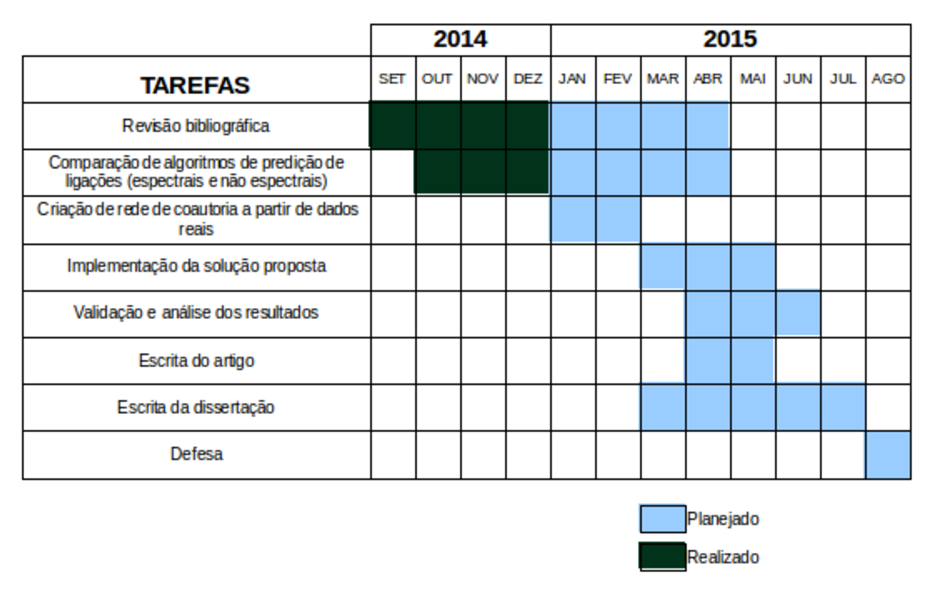
\includegraphics[width=0.9\textwidth]{cronograma.eps}
	\caption{Cronograma da Proposta de Disserta\c{c}\~{a}o.}
	\label{fig:cronograma}
\end{figure}





% -----
% PARTE DE REFERÊCIAS BIBLIOGRÁFICAS DA DISSERTAÇÃO
%
%  As referências da Proposta de Dissertação devem estar no arquivo refs.bib
%  Devem seguir o formato bibtex - ver Manual-Referencias.pdf para mais detalhes.
% -----
\bibliographystyle{proposta}
\bibliography{ref}


% -----
% PARTE DE ASSINATURAS DE SUA PROPOSTA DE DISSERTAÇÃO
% -----
\preparatitulos
\makeassinaturas


% -----
% FIM DO DOCUMENTO DE SUA PROPOSTA DE DISSERTAÇÃO
% -----
\label{theend}
\end{document}
